%!TEX encoding = UTF-8 Unicode
%!TEX root = ../compendium.tex

\chapter{Terminalfönster och kommandoskal}\label{appendix:terminal}

\section{Vad är ett terminalfönster?}

I ett terminalfönster kan man skriva kommandon som kör program och hanterar filer. När man programmerar använder man ofta terminalkommando för att kompilera och exekvera sina program.  
 
\subsubsection{Terminal i Linux}

    \begin{figure}[!b]
    \centering
    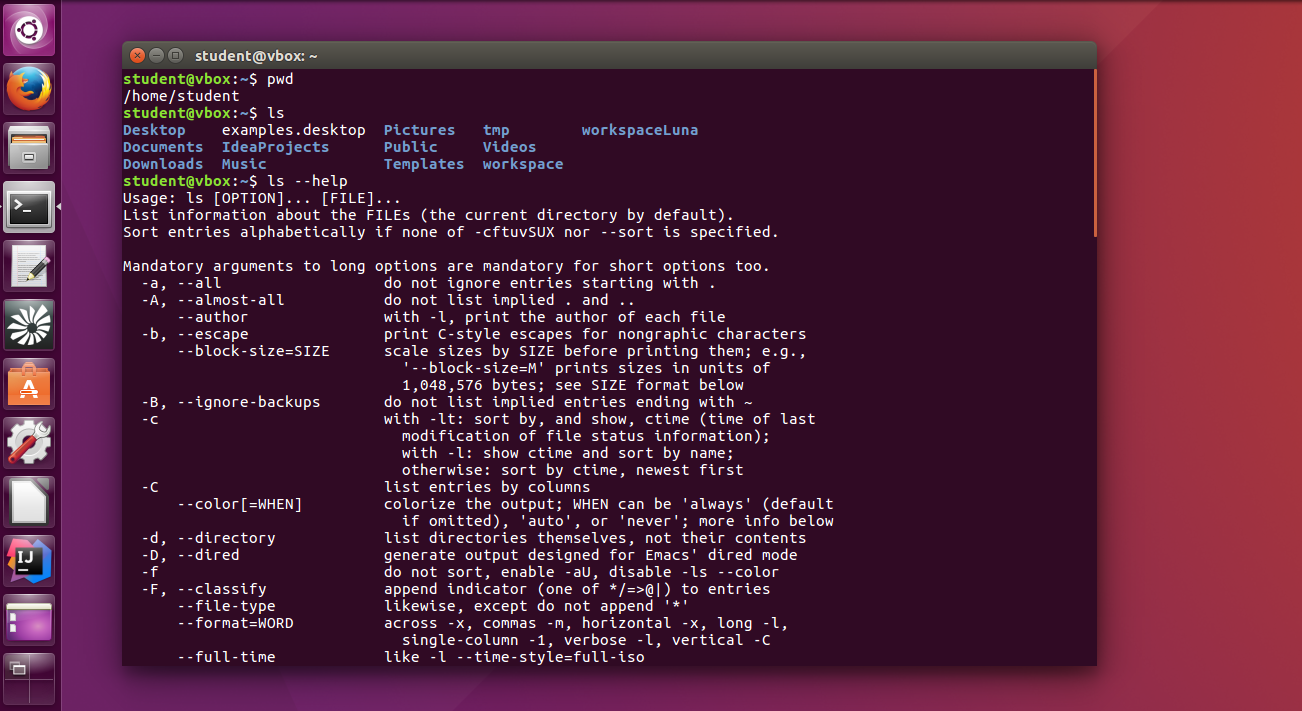
\includegraphics[width=1.0\textwidth]{../img/linux-terminal.png}
    \caption{Terminalfönster i Ubuntu öppnas med Ctrl+Alt+T.}
    \label{fig:terminal:linux}
    \end{figure}

I Linux används ofta kortkommando för att starta ett terminalfönster. I Ubuntu trycker man Ctrl+Alt+T.  Då öppnas ett fönster med en blinkande markör som visar att det är redo att ta emot dina textkommando. Ett exempel på kommando är \texttt{ls} som skriver ut en lista med filer i det aktuella biblioteket, så som visas i fig. \ref{fig:terminal:linux}.

Det som visas i ett terminalfönster sköts av ett \textbf{kommandoskal} \Eng{command shell}, som är redo att ta emot kommando efter en prompt som slutar med ett \texttt{\$}-tecken. När du skriver ett kommando och trycker Enter anropar kommandoskalet en kommandotolk som tolkar och utför dina kommandon. Om ett kommando inte kan tolkas, skrivs ett felmeddelande. Det finns ett flera användbara kortkommando som är bra att lära sig utantill, se tabell \ref{fig:terminal:shortcuts}. Det är bra om du lär dig dessa kortkommandon utantill så att ditt arbete i terminalen går snabbt och smidigt.

\begin{table}[H]
\renewcommand{\arraystretch}{1.15}
\begin{tabular}{@{}r | l}
Ctrl+A & flytta markören till början av raden \\
Ctrl+E & flytta markören till slutet av raden \\
Tab & ''auto-complete'', fyll i resten baserat på vad du skrivit hittills \\
Tab Tab & två tryck på Tab listar eventuella alternativ \\
Ctrl+K & ''kill'', ta bort tecken från markören till radens slut\\
Ctrl+U & ta bort tecken från markören till början av raden \\
Ctrl+Y & ''yank'', sätt in det som senast togs bort\\
Ctrl+Z & ''background'', det du senast startade görs till bakgrundskörning\\
Ctrl+L & rensa terminalfönstret\\
Ctrl+D & avsluta kommandoskalet \\
\end{tabular}
    \caption{Viktiga kortkommando i ett terminalfönster i Linux.}
    \label{fig:terminal:shortcuts}
\end{table}

Ctrl+C orsakar normalt ett avbrott av pågående process, men om du vill att Ctrl+C ska vara ''Copy'' som vanligt för att kopiera markerad text, kan du ställa om detta i terminalfönstrets inställningar, som du når genom fönstrets menyer.




 
\subsubsection{PowerShell och Cmd i Microsoft Windows}
Microsoft Windows är inte Linux-baserat, men i kommandotolken PowerShell finns alias definierade för några vanliga Linux-kommandon, inkluderat \texttt{ls}, \texttt{cd} och \texttt{pwd}. Du startar Powershell t.ex. genom att trycka på Windows-knappen och skriva \texttt{powershell}. Du kan också, medan du bläddrar bland filer, klicka på filnamnsraden överst i filbläddraren och skriva \texttt{powershell} och tryck Enter.

Det finns även i Windows den ursprungliga kommandotolken Cmd med helt andra kommandon. Till exempel skriver man i Cmd \texttt{dir} i stället för \texttt{ls}. 



\subsubsection{Terminal i Apple OS X / macOS}
Apple OS X och macOS är Unix-baserade operativsystem. De flesta vanliga terminalkommandon som fungerar i Linux fungerar också under Apple OS X och macOS.

\section{Några viktiga terminalkommando}

Tipsa om \href{http://ss64.com/}{ss64.com} och \url{http://www.ddg.lth.se/perf/unix/}